\chapter{Métodos semânticos de dedução na lógica proposicional}


Capítulo 4 de Souza, \textit{Lógica para Ciência da Computação}~\cite{souza_logica_3}.

\vspace{1cm}


%%%%%%%%%%%%%%%%%%%%%%%%%%%%%%%%%%%%%%%%%%%%%%%%%%%%%%%%%%%%
\section{Introdução}

\begin{easylist}
  & Validade de fórmulas: uma fórmula é válida sse todas as suas interpretações são iguais a $V$.
\end{easylist}


%%%%%%%%%%%%%%%%%%%%%%%%%%%%%%%%%%%%%%%%%%%%%%%%%%%%%%%%%%%%
\section{Método da tabela verdade}

\begin{easylist}
  & Método da tabela verdade: é um método exaustivo, ou seja, enumera todas as possibilidades. A desvantagem é que, se houver muitos símbolos proposicionais, a tabela fica muito grande.
  & Exemplo: seja $H = \; \NOT(P \AND Q) \BIC (\NOT P \OR \NOT Q)$, demonstre que $H$ é uma tautologia usando o método da tabela verdade.  
\end{easylist}

\begin{center}
  \begin{tabular}{ c|c|c|c|c|c|c|c }
    $P$ & $Q$ & $\NOT P$ & $\NOT Q$ & $(P \AND Q)$ & $\NOT(P \AND Q)$ & $(\NOT P \OR \NOT Q)$ & $H$ \\
    \hline
    $T$ & $T$ & $F$      & $F$      & $T$          & $F$              & $F$                   & $T$ \\
    $T$ & $F$ & $F$      & $T$      & $F$          & $T$              & $T$                   & $T$ \\
    $F$ & $T$ & $T$      & $F$      & $F$          & $T$              & $T$                   & $T$ \\
    $F$ & $F$ & $T$      & $T$      & $F$          & $T$              & $T$                   & $T$ \\
  \end{tabular}
\end{center}

%%%%%%%%%%%%%%%%%%%%%%%%%%%%%%%%%%%%%%%%%%%%%%%%%%%%%%%%%%%%
\section{Método da negação ou absurdo}

\begin{easylist}
  & Método da negação ou absurdo: funciona da seguinte maneira.
  && Faça uma suposição.
  && Se todas as substituições possíveis levarem a contradições, a suposição é falsa. Ou seja, a negação da suposição é verdadeira.

  & Exemplo: seja $H = \; ((P \IMP Q) \AND (Q \IMP R)) \IMP (P \IMP R)$, demonstre por absurdo que $H$ é uma tautologia.
  && Demonstração: assuma por absurdo que existe interpretação $I$ tal que $I(H) = F$.

  Então $I((P \IMP Q) \AND (Q \IMP R)) = T$ e
  $I(P \IMP R) = F$.

  Como $I(P \IMP R) = F$, então $I(P) = T$ e $I(R) = F$.

  Distribuindo na fórmula os valores de verdade encontados, temos

$    (( P \IMP Q) \AND (Q \IMP R)) \IMP (P \IMP R)    $

$ \;\;\;    T \hspace{30pt} T \hspace{30pt} F \hspace{10pt} F \;\;\; T \; F \; F  $

de onde obtemos

$    (( P \IMP Q) \AND (Q \IMP R)) \IMP (P \IMP R)    $

$ \;\;\;    T \;\; T \; T \;\; T \;\; F \;\; T \;\; F \hspace{10pt} F \;\;\; T \; F \; F  $

$ \hspace{32pt} \uparrow \hspace{21pt} \uparrow $

\hspace{18pt} Contradição

Portanto, a suposição inicial de que existe interpretação $I$ tal que $I(H) = F$ é falsa. Em outras palavras, para todo $I$, $I(H)=T$, ou seja, $H$ é tautologia.

\end{easylist}


%%%%%%%%%%%%%%%%%%%%%%%%%%%%%%%%%%%%%%%%%%%%%%%%%%%%%%%%%%%%
\section{Método da árvore semântica}

\begin{easylist}
  & Método da árvore semântica: é um método que permite a verificação da validade de uma fórmula sem ser exaustivo. A depender da fórmula, pode ser possível obter a resposta sem verificar todas as interpretações possíveis. Este conteúdo está na primeira edição do livro de Souza \textit{Lógica para Ciência da Computação}~\cite{souza_logica_1}.

\clearpage
  
  & Exemplo: seja $H = \; \NOT(P \AND Q) \BIC (\NOT P \OR \NOT Q)$, demonstre que $H$ é uma tautologia usando o método da árvore semântica.
\end{easylist}

\begin{center}
  \begin{tabular}{ c|cccccccccc }
        & $\NOT$ & $(P$ & $\AND$ & $Q)$ & $\BIC$ & $(\NOT$ & $P$ & $\OR$ & $\NOT$ & $Q)$ \\
    \hline
      2 &        & $T$  &        &      &        & $F$     & $T$ &       &        &      \\
    \hline
      3 & $T$    & $F$  & $F$    &      & $T$    & $T$     & $F$ & $T$   &        &      \\
    \hline
      4 & $F$    & $T$  & $T$    & $T$  & $T$    & $F$     & $T$ & $F$   & $F$    & $T$  \\
    \hline
      5 & $T$    & $T$  & $F$    & $F$  & $T$    & $F$     & $T$ & $T$   & $T$    & $F$  \\
  \end{tabular}
\end{center}

\begin{figure}[h!]
  \begin{center}
    \begin{tabular}{c}
      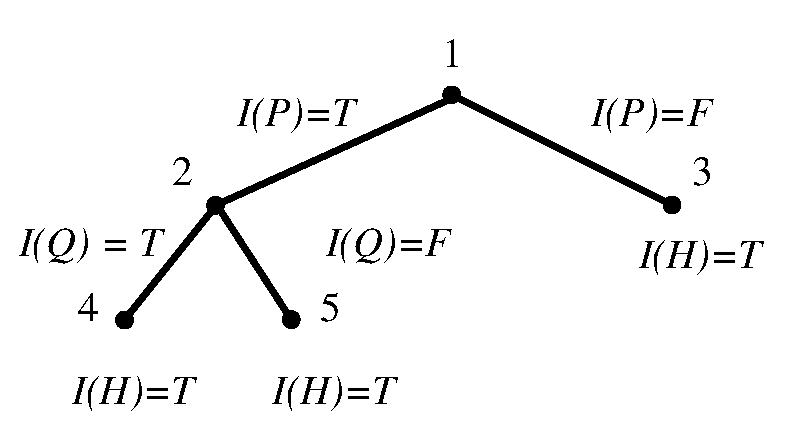
\includegraphics[width=0.7\textwidth]{images/04/tree_01.eps}
    \end{tabular}
  \end{center}
  %\caption{\label{fig:tree:01}}
\end{figure}

%\clearpage

\begin{easylist}
  & Exemplo: seja $H = \; (P \OR \NOT Q) \BIC (\NOT P \IMP \NOT Q)$, demonstre que $H$ é uma tautologia usando o método da árvore semântica.
\end{easylist}

\begin{center}
  \begin{tabular}{ c|cccccccccc }
        & $(P$ & $\OR$ & $\NOT$ & $Q)$ & $\BIC$ & $(\NOT$ & $P$ & $\IMP$ & $\NOT$ & $Q)$ \\
    \hline
      2 & $T$  & $T$   &        &      & $T$    & $F$     & $T$ & $T$    &        &      \\
    \hline
      3 & $F$  &       &        &      &        & $T$     & $F$ &        &        &      \\
    \hline
      4 & $F$  & $F$   & $F$    & $T$  & $T$    & $T$     & $F$ & $F$    & $F$    & $T$  \\
    \hline
      5 & $F$  & $T$   & $T$    & $F$  & $T$    & $T$     & $F$ & $T$    & $T$    & $F$  \\
  \end{tabular}
\end{center}

\begin{figure}[h!]
  \begin{center}
    \begin{tabular}{c}
      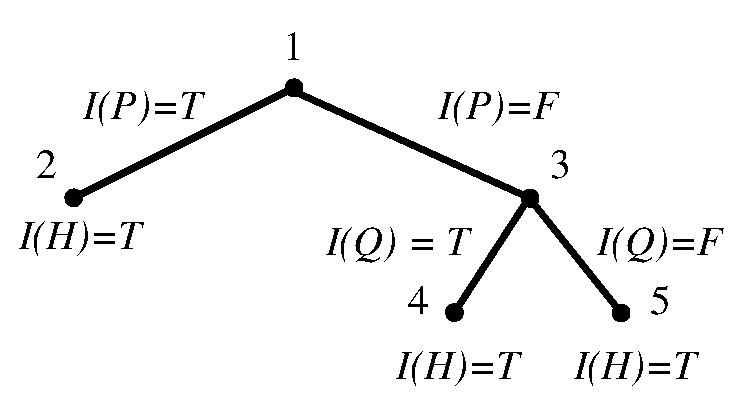
\includegraphics[width=0.7\textwidth]{images/04/tree_02.eps}
    \end{tabular}
  \end{center}
  %\caption{\label{fig:tree:01}}
\end{figure}


%%%%%%%%%%%%%%%%%%%%%%%%%%%%%%%%%%%%%%%%%%%%%%%%%%%%%%%%%%%%
\section{Método do tableaux semântico}

\begin{easylist}
  & Tableaux semântico: sequência de fórmulas construída de acordo com um conjunto de regras e apresentada em forma de árvore. O método de tableaux semânticos é um mecanismo de decisão para a pergunta $\beta \vdash H$, sim ou não?

  & Elementos do sistema de tableaux semânticos da lógica proposicional:
  && Alfabeto da lógica proposicional sem os símbolos de verdade $\TRUE$ e $\FALSE$.
  && Conjunto das fórmulas da lógica proposicional.
  && Um conjunto de regras de dedução.

  & Regras de dedução do tableau semântico: sejam $A$ e $B$ duas fórmulas da lógica proposicional, as regras de dedução do sistema de tableaux semânticos são

\begin{figure}[h!]
  \begin{center}
    \begin{tabular}{c}
      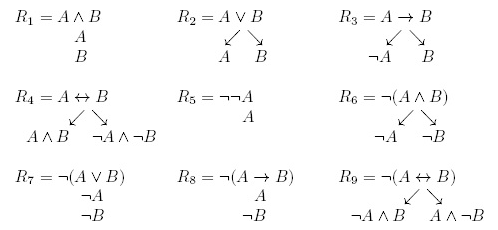
\includegraphics[width=0.7\textwidth]{images/04/tableaux.png}
    \end{tabular}
  \end{center}
  %\caption{\label{fig:tree:01}}
\end{figure}

  & Construção de um tableau semântico: se dá aplicando alguma regra de dedução uma vez para cada linha que não seja um literal (símbolo proposicional ou sua negação). O tableau resultante tende a ficar mais simples se aplicarmos primeiro as regras de dedução que não geram bifurcações $(R_1, R_5, R_7, R_8)$.
  && Exemplo: considere o conjunto de fórmulas: $\{A \IMP B, \NOT(A \OR B),  \NOT (C \IMP A)\}$. Encontre o tableau semântico iniciado com esse conjunto de fórmulas.

\end{easylist}

%\forestset{%
%  vertical/.style={                       %define style for phantom node
                                          %with vertical edge drawn from it
%    before drawing tree={not ignore edge, edge=draw},
%  },
%}

%\begin{tableau}
%  {line no sep= 1.5cm,
%    just sep= 1.5cm,
%    for tree={s sep'=10mm},
%    close with=\absurd
%}
%  [((P \land Q) \lor R),                   just={Premiss}
%    [\neg\neg(\neg P \lor \neg R),       just={Negated conclusion}
%      [(\neg P \lor \neg R),           just={From (2)}
%        [(P \land Q),                just={Alternatives from (1)}
%          [P,                      just={From (4)}
%            [Q,                  just={From (4)}
%              [\neg P,close]
%              [\neg R,         just={Alternatives from (3)}
%        ]]]]
%        [R
%          [, vertical               %phantom node but with edge
%            [, vertical       %phantom node but with edge
%              [\neg P]          %and now we have two
%              [\neg R,close]    %brances added
%  ]]]]]]
%\end{tableau}

\iffalse

\forestset{%
  vertical/.style={     %define style for phantom node
                        %with vertical edge drawn from it
    before drawing tree={not ignore edge, edge=draw},
  },
}

\begin{tableau}
{                              % begin tree preamble
    line no sep= 2cm,          % distance of tree from line numbers
    just sep= 1.5cm,
    for tree={s sep'=10mm},    % control horizontal spread of branches
}                              % end tree preamble
  [P
    [(P \IMP Q)                just={From 1.}
      [\NOT Q                  just={From 1.}
        [\NOT P, close]        just={From 1.}
        [Q, close]             just={From 1.}
      ]                        just={From 1.}
    ]                          just={From 1.}
  ]
\end{tableau}

\fi


\begin{prooftree}
  {
    to prove={\{P \OR (Q \OR \NOT R), P \IMP\NOT R, Q \IMP \NOT R\}
      \vdash{}{} \NOT R ~P \text{\~{}}P}
  }
  [P \OR (Q \OR \NOT R), just=Ass, checked
    [P \IMP \NOT R, just=Ass, checked
      [Q \IMP \NOT R, just=Ass, checked,name=last premise
        [\NOT\NOT R, just={$\NOT$ Conc},name=not conc
          [P, just={$\OR$ Elim:!uuuu}
            [\NOT P, close={:!u,!c}]
            [\NOT R, close={:not conc,!c},just={$\IMP$ Elim:!uuuu}]
          ]
          [Q \OR \NOT R
            [Q, move by=1
              [\NOT Q, close={:!u,!c}]
              [\NOT R, close={:not conc,!c},just={$\IMP$ Elim:last premise}]
            ]
            [\NOT R, close={:not conc,!c},move by=1, just={$\OR$ Elim:!u}]
          ]
        ]
      ]
    ]
  ]
\end{prooftree}



\clearpage

\begin{easylist}

& Ramo: é uma sequência de fórmulas onde cada fórmula é derivada das anteriores através das regras de dedução. A primeira fórmula do ramo é sempre a primeira fórmula do tableau.

& Ramo fechado: é um ramo que contém uma fórmula e sua negação.

& Ramo saturado: é um ramo onde, para todas as suas fórmulas,
&& já foi aplicada alguma regra de dedução; ou
&& não é possível aplicar nenhuma regra de derivação, isto é, a fórmula é um literal.

& Ramo aberto: é um ramo saturado não fechado.

& Tableau fechado: é um tableau onde todos os ramos são fechados.

& Tableau aberto: é um tableau onde algum ramo é aberto.

& Prova de $H$ no sistema de tableaux semânticos: é um tableau fechado iniciado com a fórmula $\NOT H$
&& Exemplos: verifique se as fórmulas abaixo são tautologias:
&&& $ \NOT((P \IMP Q) \AND \NOT (P \BIC Q) \AND \NOT\NOT P) $
&&& $ (P \BIC Q) \OR \NOT P $

&& Pergunta: um tableau iniciado com uma tautologia necessariamente terá todos os ramos abertos?
&&& Resposta: não. Um contra-exemplo é a fórmula $ (P \AND \NOT P) \OR (Q \IMP Q) $

\end{easylist}

%%%%%%%%%%%%%%%%%%%%%%%%%%%%%%%%%%%%%%%%%%%%%%%%%%%%%%%%%%%%
\section{Exercícios}

%$ \NOT \; \OR \; \AND \; \IMP \; \BIC$

\begin{enumerate}
  \item Determine por absurdo se as fórmulas a seguir são ou não tautologias.
    \begin{enumerate}
      \item $H_1 = \NOT(\NOT H) \BIC H$
      \item $H_2 = \NOT(H \IMP G) \BIC (\NOT H \BIC G)$
      \item $H_3 = \NOT(H \BIC G) \BIC (\NOT H \BIC G)$
      \item $H_4 = (H \BIC G) \BIC ((H \IMP G) \AND (G \IMP H))$
      \item $H_5 = (H \AND (G \OR E)) \BIC ((H \AND G) \OR (H \AND E))$
      \item $H_6 = ((H \IMP G) \AND (G \IMP H) \IMP (H \IMP H)$
      \item $H_7 = ((H \BIC G) \AND (G \BIC H) \IMP (H \BIC H)$
      \item $H_8 = H \IMP (H \AND G)$
    \end{enumerate}
\end{enumerate}
